\documentclass{scribe-cgenomics}
\usepackage{float}
\usepackage{subfig}

\begin{document}

\جلسه
{دکتر مجتبی تفاق، ترم دوم سال تحصیلی ۱۴۰۱}
{پروژه درس بهینه‌سازی در علوم داده}
{محسن قدرتی، محمد صالح بهرامی}


\section{مقدمه}


\section{تعاریف اولیه}
\subsection{مدل‌های اتوریگرسیو}
\subsection{فیلتر}


\section{معرفی مساله داده‌کاوی}
\subsection{صورت مساله و داده‌ها}
\subsection{تخمین حافظه موثر}
\subsection{تخمین سایز مناسب برای یادگیری دینامیک مساله}
\subsection{تهیه تعدادی ویژگی (کنترل دینامیک)}


% --------------------------------------------- %
\section{فیلتر کالمن}
% --------------------------------------------- %
% >>
\subsection{تعریف}

% >>
\subsection{الگوریتم}


% >>
\subsection{تحلیل زمانی}


% >>
\subsection{پیاده‌سازی}

\subsubsection{مدل ۱: دینامیک خطی بدون کنترل}
فرض می‌کنیم دینامیک تغییرات قیمت به شکل زیر باشد:
\begin{equation}\label{linear_model_without_control}
\tilde{r}_n = f_{0, n}\tilde{r}_{n-1} + \sum_{i=1}^{m-1}f_{i, n} r_{i,n-1} + f_{m, n} + w_n,
\qquad
w_n \sim \mathcal{N}(0,\ \sigma_n^{2}) \..
\end{equation}
به عبارت دیگر، فرض می‌کنیم اگر تغییرات قیمت از
$i = 2,\ \dots,\ m-1$
کندل گذشته تا کندل گذشته را بدانیم و تغییرات قیمت از کندل گذشته تا کندل فعلی را نیز بدانیم، بازدهی پیش رو ترکیبی خطی از این مقادیر به علاوه یک نویز با توزیع نرمال است.
در این صورت برای بردار
$\bold{x^{(n)}}$
فرم معادل زیر را خواهیم داشت:

\begin{equation}
\bold{x^{(n)}} = F_n\bold{x^{(n-1)}} + \bold{w^{(n)}},
\end{equation}

که در آن
\begin{center}
$
\bold{x^{(n)}} := 
\begin{bmatrix}
\tilde{r}_n \\
r_{1, n} \\
\vdots \\
r_{m-1, n} \\
1
\end{bmatrix},
\quad 
F_n := 
\begin{bmatrix}
f_{0, n} & f_{1, n} & \dots & f_{m, n} \\
1 + \tilde{r}_{n-1} & 0 & \ddots & 0 \\
0 & 1 + \tilde{r}_{n-1} & 0 & \vdots \\
0 & \ddots &  & 0 \\
\vdots & 0  & 1 + \tilde{r}_{n-1} & 0 \\
0 & \dots & 0 & 1
\end{bmatrix},
\quad
\bold{w^{(n)}} := 
\begin{bmatrix}
w_n \\
-{\tilde{r}_{n-1}}^2 \\
\tilde{r}_{n-1} \\
\vdots \\
\tilde{r}_{n-1} \\
0
\end{bmatrix}\..
$
\end{center}
با توجه به این که در هر لحظه
$n$، 
بردار
$\bold{x^{(n-1)}}$
معلوم است و کواریانس بردار
$\bold{w^{(n)}}$
تنها در درایه
$1,1$
ناصفر و برابر با
$\sigma_n^2$
است، به دنبال مقادیری از
$f_{0, n},\ \dots,\ f_{m-1, n}$
می‌گردیم که
$\sigma_n^2$
را کمینه کند. (در واقع خطای مدل را در حد امکان کاهش دهد.) هم‌چنین توجه می‌کنیم که اضافه کردن عدد
$1$
به انتهای بردار
$\bold{x^{(n)}}$
باعث می‌شود بتوان عرض از مبدا مدل
\ref{linear_model_without_control}
را به
$f_{m,n}$
منتقل کرد و لذا فرض صفر بودن میانگین نویز
$w_n$
برقرار است. اکنون سعی می‌کنیم با بازنویسی معادله بالا، فرم مجموع مربعاتی برای یافتن بهترین
$f_{i,n}$ها
ارایه کنیم.

اگر قرار دهیم
$\theta_n = (f_{0,n},\ \dots,\ f_{m, n})^T$،
به دنبال حل مساله بهینه‌سازی زیر هستیم:
\begin{center}
$minimize_{(\theta_n)}\quad |\tilde{r}_n - \langle\theta_n,\ \bold{x^{(n-1)}}\rangle |^2$
\end{center}
اما با توجه به اینکه مساله بالا احتمالا بی‌نهایت جواب دارد و این موضوع باعث تغییرات سریع دینامیک مدل در هر لحظه می‌شود که خلاف طبیعت مدل است، و مهم‌تر آنکه انتظار داریم دینامیک مدل در طول یک پنجره کوتاه مدت
($k$تایی)
پایدار باشد (یعنی
$\theta_{n}\simeq \theta_{n-1} \simeq \dots \simeq \theta_{n-(k-1)}$) و بتوانیم از اطلاعات این پنجره برای تقریب یک دینامیک کم‌نوسان بهره ببریم، مساله بهینه‌سازی فوق را به مساله زیر تعمیم می‌دهیم:
\begin{center}
$minimize_{(\theta_n)} \quad |\tilde{r}_{n-(k-1)} - \langle\theta_{n},\ \bold{x^{(n-1-(k-1))}}\rangle |^2 + \dots + |\tilde{r}_n - \langle\theta_n,\ \bold{x^{(n-1)}}\rangle |^2$
\end{center}
که با در نظر گرفتن ماتریس
$X^{(n)}$
به صورت
\begin{center}
$
X^{(n)} = 
\begin{bmatrix}
\bold{x^{(n-(k-1))}}^T \\
\vdots \\
\bold{x^{(n)}}^T \\
\end{bmatrix}
\quad
\rightarrow
\quad
X^{(n)} :=
\begin{bmatrix}
\bold{b^{(n)}_0} & \dots & \bold{b^{(n)}_m}
\end{bmatrix}
$
\end{center}
به فرم زیر قابل بیان است:
\begin{equation}\label{linear_model_without_control_optimization}
for\ given\ n:\quad minimize_{(\theta_n)}\ ||X^{(n-1)}\theta_n - \bold{b^{(n)}_0}||_2^2
\end{equation}
توجه به این نکته ضروری است که از بردار
$X^{(n)}_0$،
درایه اول مربوط به بازدهی آینده است و در درسترس نیست. لذا به جای حل مساله فوق برای
$n$
آن را برای
$n-1$
حل می‌کنیم.

در ادامه به بررسی نتایج حاصل از حل مساله بهینه‌سازی
\ref{linear_model_without_control_optimization}
به کمک روش کمترین مجموع مربعات و پیاده‌سازی فیلتر کالمن بر روی مدل
\ref{linear_model_without_control}
می‌پردازیم.

\begin{مشاهده}
مطابق با نمودار زیر می‌توان فرض نرمال بودن نویز در اندازه‌گیری و مدل را تا حدودی تایید کرد. هم‌چنین توجه می‌کنیم که میانگین توزیع نویز، با دقت ۷ رقم اعشار صفر خواهد بود.

\begin{figure}[h]
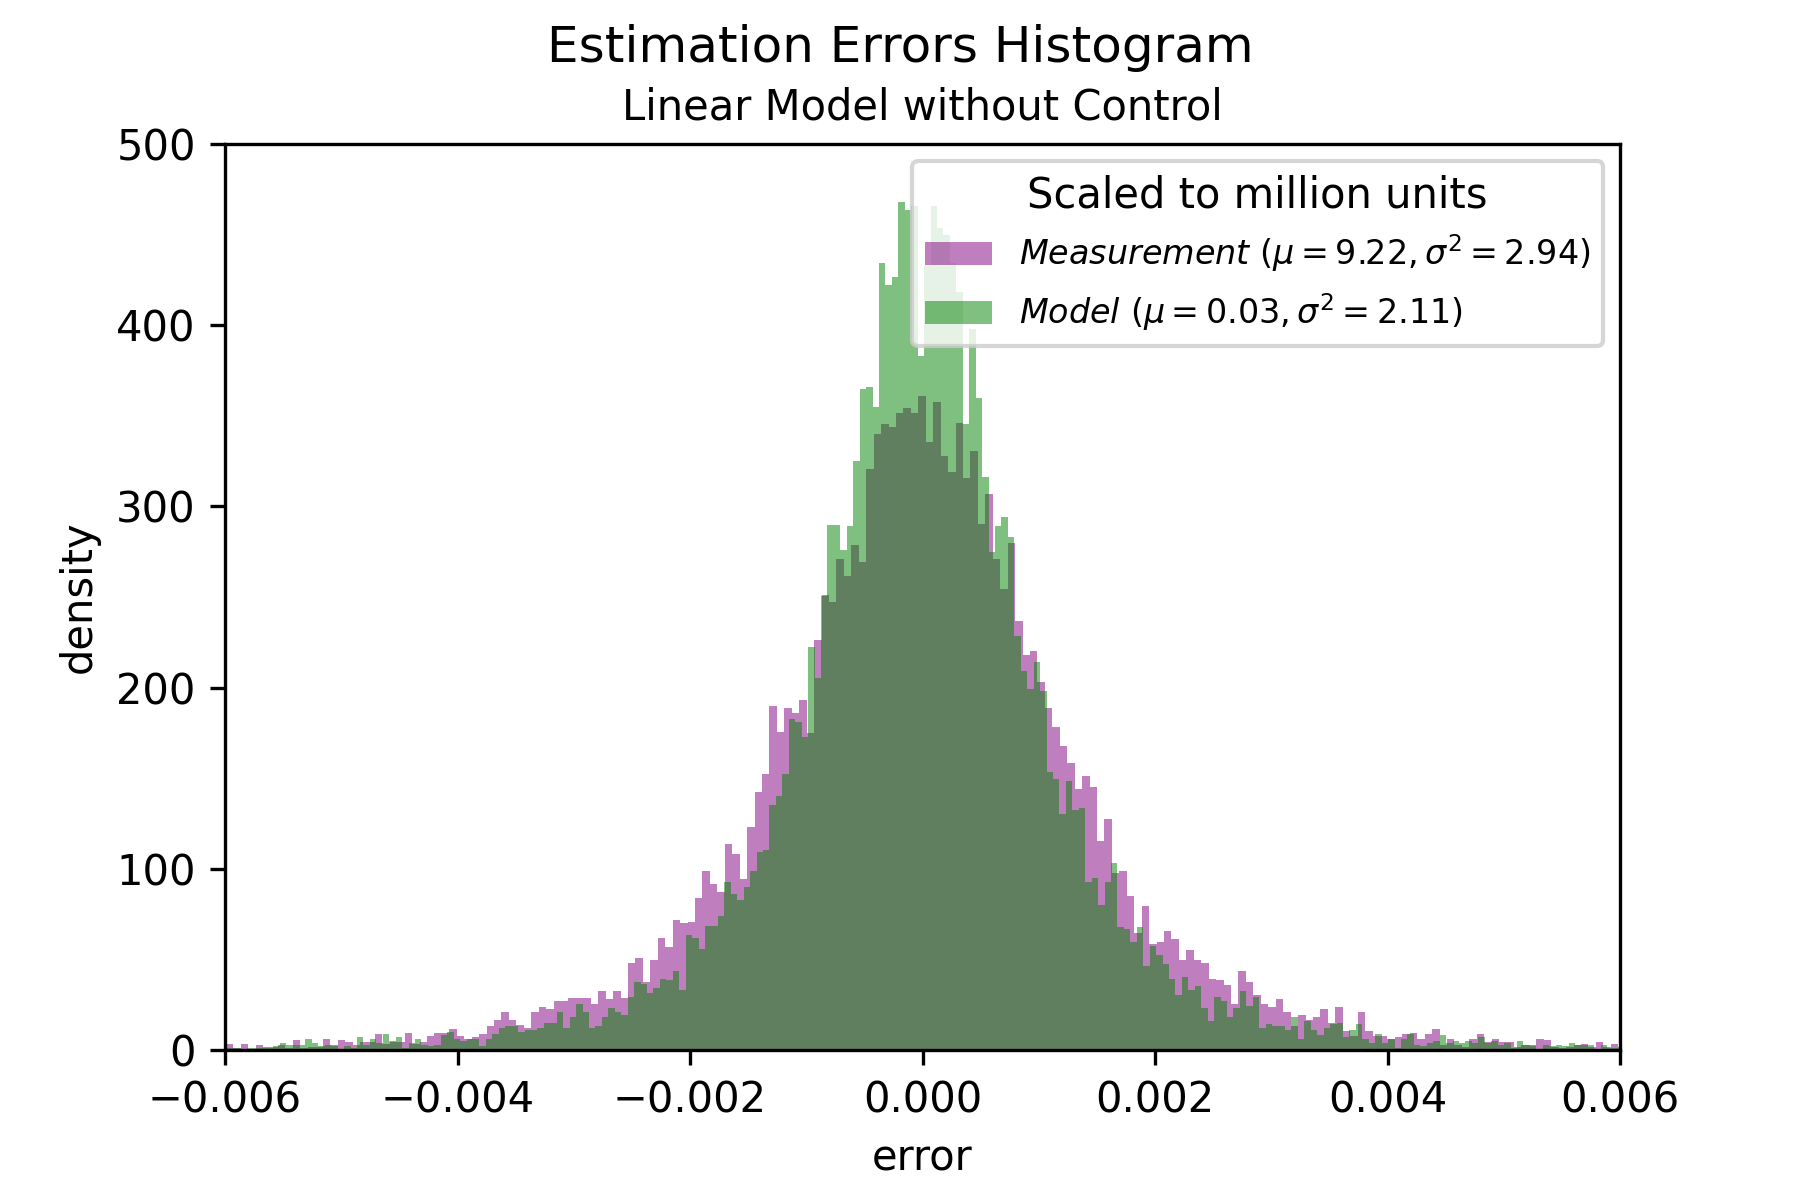
\includegraphics[width=0.5\textwidth]{Errors Histogram [Linear Model without Control].png}
\centering
\end{figure}
\end{مشاهده}

\begin{مشاهده}
همان‌طور که اشاره کردیم، فرض می‌کنیم دینامیک مدل دچار تغییرات سریع نمی‌شود. این نکته در نمودار زیر به صورت طیف‌های پیوسته قابل مشاهده است. هم‌چنین در نمودار زیر این نکته قابل توجه وجود دارد که ضرایب بزرگ‌تر و تاثیرگذارتر در مدل خطی پیشنهاد شده، به لحظات نزدیک‌تر به لحظه حال مرتبط می‌شوند. این نیز مشاهده‌ای است که انتظارش را داشتیم.

\begin{figure}[h]
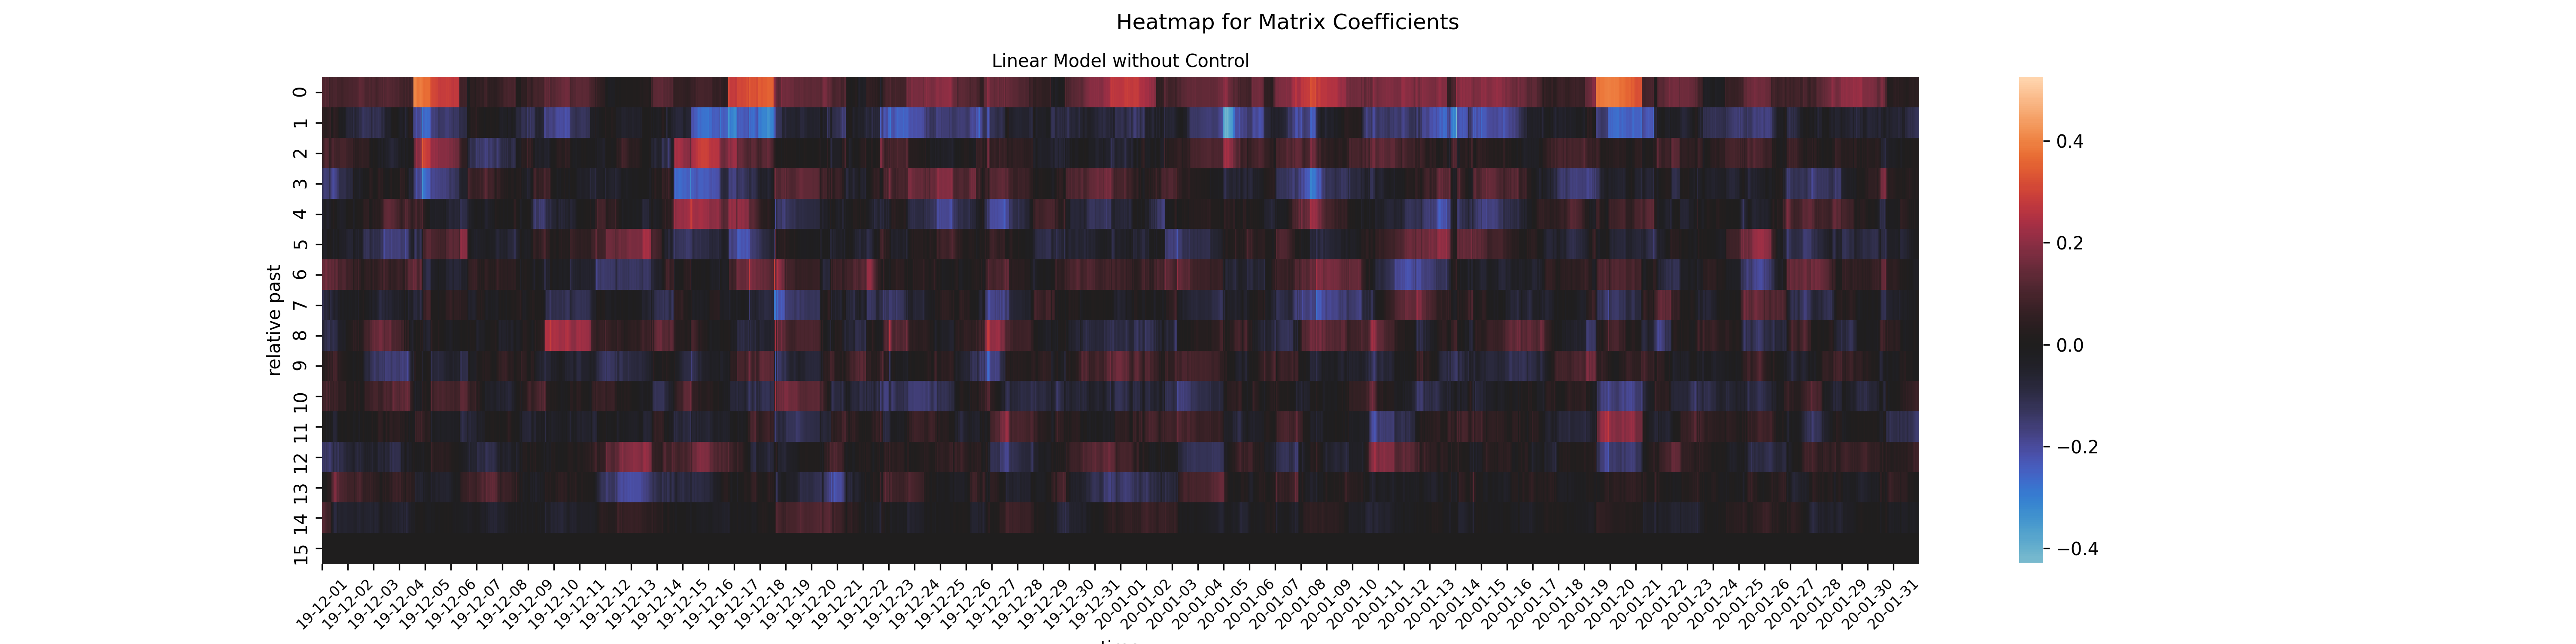
\includegraphics[width=1.1\textwidth]{Heatmap [Linear Model without Control].png}
\centering
\end{figure}
\end{مشاهده}

\begin{نتیجه}
در شکل می‌توان خروجی فیلتر کالمن را بر روی مدل خطی در هر لحظه به ازای یک پنجره خاص زمانی مشاهده کرد.

\begin{figure}[h]
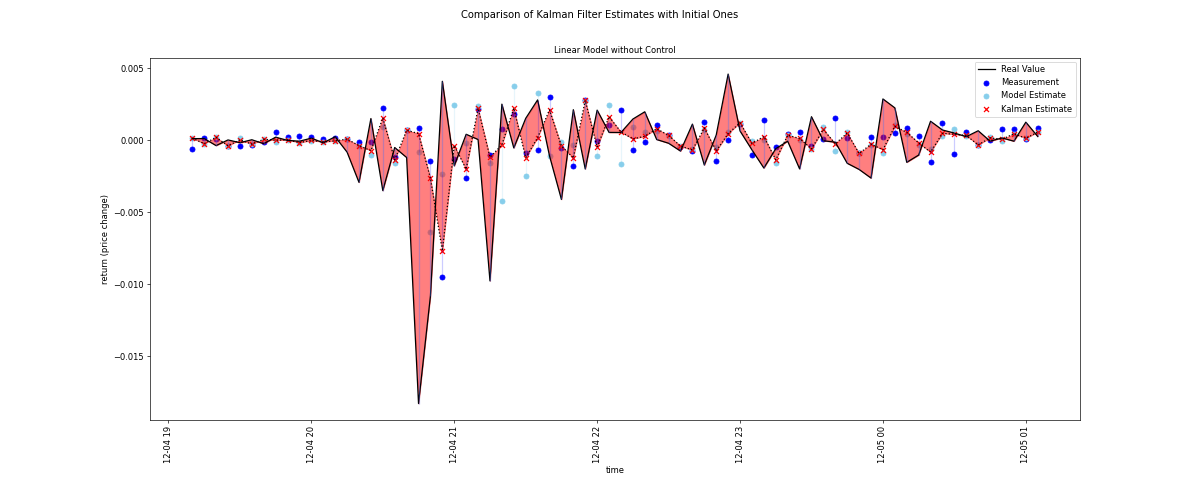
\includegraphics[width=1\textwidth]{Returns and Kalman Filtering [Linear Model without Control].png}
\centering
\end{figure}
\end{نتیجه}

\subsubsection{مدل ۲: دینامیک خطی همراه با کنترل}
در مدل زیر، فرض می‌کنیم تعدادی ویژگی (که در بخش قبل تهیه شده‌اند و در همان بخش، همبستگیشان با تابع هدف ما بررسی و تایید شده است) نیز علاوه بر بردار
$\bold{x^{(n-1)}}$،
در دینامیک تغییرات قیمت به شکل خطی موثر باشند. به عبارت دیگر دینامیک مساله را با مدل زیر تقریب می‌زنیم:

\begin{equation}\label{linear_model_with_control}
\tilde{r}_n = f_{0, n}\tilde{r}_{n-1} + \sum_{i=1}^{m-1}f_{i, n} r_{i,n-1} + f_{m, n} + \sum_{i=0}^{s-1}g_{i,n}u_{i,n} + w_n,
\qquad
w_n \sim \mathcal{N}(0,\ \sigma_n^{2}) \..
\end{equation}

که با فرم زیر معادل است:

\begin{equation}
\bold{x^{(n)}} = F_n\bold{x^{(n-1)}} + G_n\bold{u^{(n)}} + \bold{w^{(n)}},
\end{equation}

و در آن
$\bold{u^{(n)}}$
بردار ویژگی‌ها در لحظه
$n$
است. در واقع:

\begin{center}
$
G_n := 
\begin{bmatrix}
g_{0, n} & \dots & g_{s-1, n} \\
0 & \dots & 0 \\
 & \ddots & \\
0 & \dots & 0
\end{bmatrix},
\quad 
\bold{u^{(n)}} := 
\begin{bmatrix}
u_{0, n} \\
\vdots \\
u_{s-1, n}
\end{bmatrix}\..
$
\end{center}

با در نظر گرفتن ماتریس
$X^{(n)}$
و بردار
$\bold{b^{(n)}_0}$
مدل قبلی، و تعریف ماتریس
$U_{n}$
و بردار
$\theta'_n$
به شکل زیر،

\begin{center}
$
U_{n} := 
\begin{bmatrix}
\bold{u^{(n - (k-1))}}^T \\
\vdots \\
\bold{u^{(n)}}^T \\
\end{bmatrix},
\qquad
\theta'_n :=
\begin{bmatrix}
g_{0,n} \\
\vdots \\
g_{s-1,n}
\end{bmatrix}
$
\end{center}

می‌توان به سادگی و مشابه با روند مدل
\ref{linear_model_without_control}،
به مساله کمترین مجموع مربعات زیر دست یافت:

\begin{equation}\label{linear_model_with_control_optimization}
for\ given\ n:\quad minimize_{(\theta_n, \theta'_n)}\ ||X^{(n-1)}\theta_n + U_{n}\theta'_n - \bold{b^{(n)}_0}||_2^2
\end{equation}

اکنون با ادغام دو ماتریس
$X^{(n-1)}$
و
$U_n$
و ادغام دو بردار
$\theta_n$
و
$\theta'_n$
مساله بهینه‌سازی معادل زیر را داریم:

\begin{center}
$
A_n := 
\begin{bmatrix}
X^{(n-1)} & U_n
\end{bmatrix},
\quad
\theta^*_n :=
\begin{bmatrix}
\theta_n \\
\theta'_n
\end{bmatrix}
\qquad
\longrightarrow
\qquad
for\ given\ n:\quad minimize_{(\theta^*_n)}\ ||A_n\theta^*_n - \bold{b^{(n)}_0}||_2^2
$
\end{center}


در ادامه به بررسی نتایج حاصل از حل مساله بهینه‌سازی
\ref{linear_model_with_control_optimization}
به کمک روش کمترین مجموع مربعات و پیاده‌سازی فیلتر کالمن بر روی مدل
\ref{linear_model_with_control}
می‌پردازیم.

\begin{مشاهده}
مطابق با نمودار زیر می‌توان فرض نرمال بودن نویز در اندازه‌گیری و مدل را مجددا تا حدودی تایید کرد. هرچند همانطور که از نمودار پیداست، واریانس مدل کمی افزایش (جزیی) داشته و کم نشده است! در بخش‌های بعدی، زمانی که همه مدل‌های خطی را معرفی کردیم و به مقایسه عملکرد آن‌ها پرداختیم، دلیل عملیاتی این موضوع را توضیح خواهیم داد.

\begin{figure}[h]
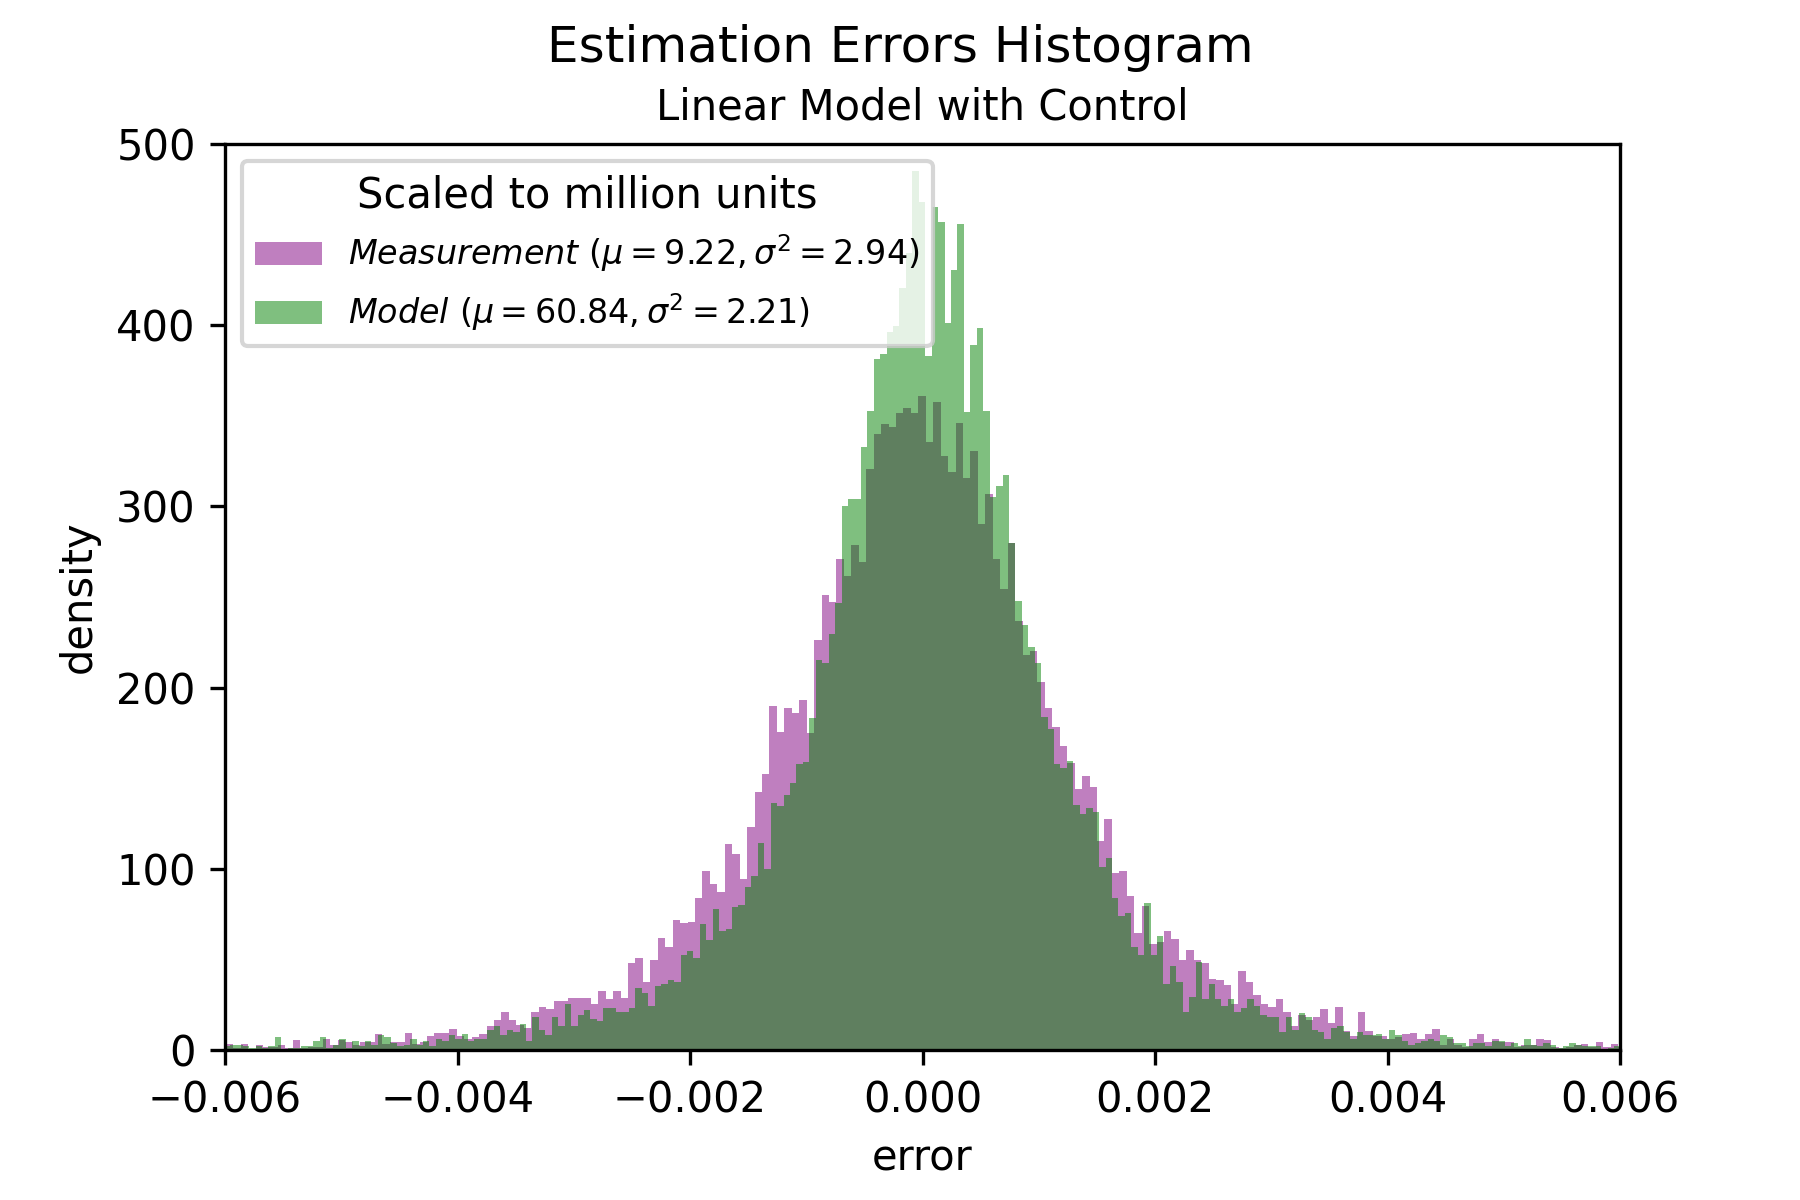
\includegraphics[width=0.5\textwidth]{Errors Histogram [Linear Model with Control].png}
\centering
\end{figure}
\end{مشاهده}


\begin{مشاهده}
نمودار زیر مشابه با نمودار مربوط به مدل
\ref{linear_model_without_control}
قابل قبول است. نکته حایز اهمیت در این نمودار، تباهیده شدن ضرایب مربوط به ویژگی‌هاست که در واقع به دلیل انحراف معیار بالاتر ستون‌های مربوط به ویژگی‌ها نسبت به ستون‌های مربوط به بازدهی است و اطلاعاتی از دست نرفته است.

\begin{figure}[h]
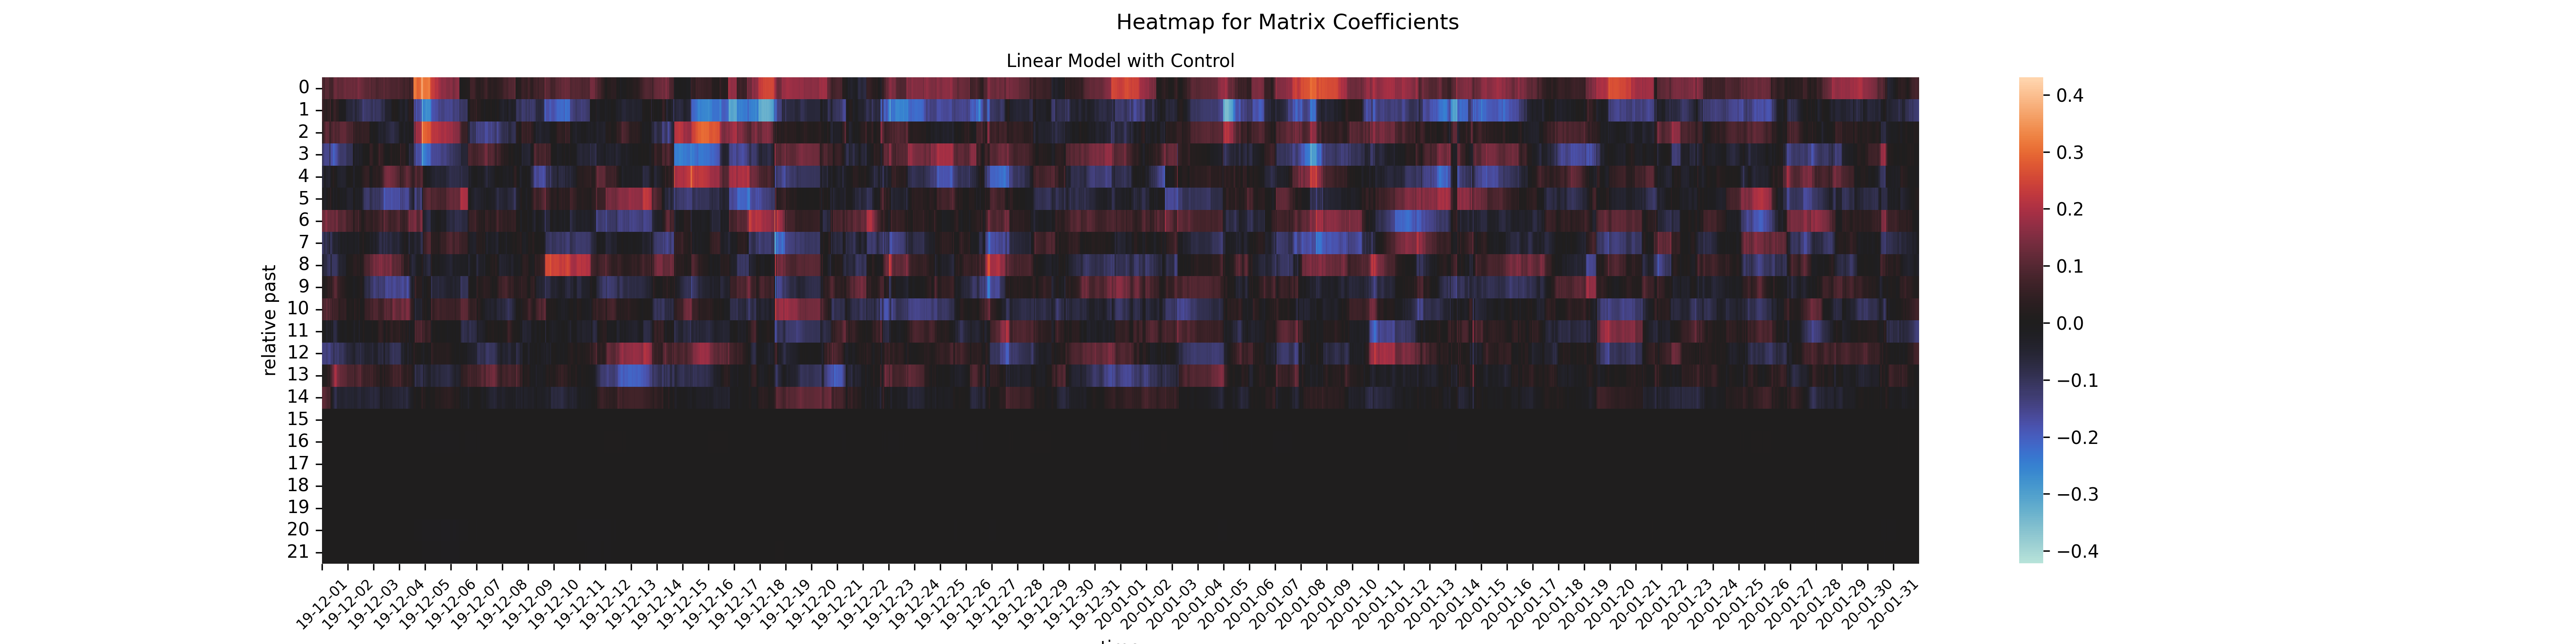
\includegraphics[width=1.1\textwidth]{Heatmap [Linear Model with Control].png}
\centering
\end{figure}
\end{مشاهده}

\begin{نتیجه}
در شکل زیر می‌توان خروجی فیلتر کالمن را بر روی مدل خطی در هر لحظه به ازای یک پنجره خاص زمانی مشاهده کرد.

\begin{figure}[h]
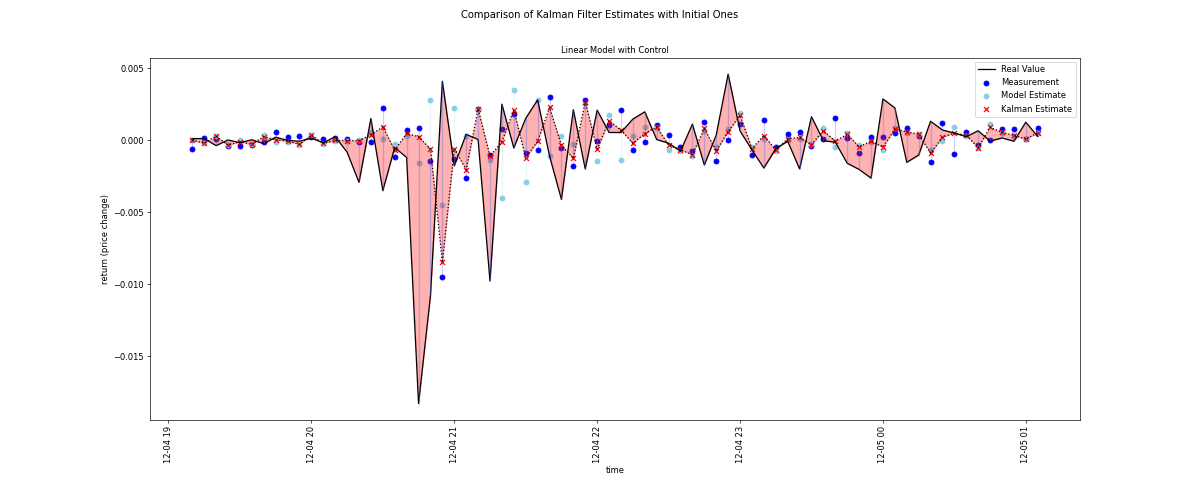
\includegraphics[width=1\textwidth]{Returns and Kalman Filtering [Linear Model with Control].png}
\centering
\end{figure}
\end{نتیجه}




\subsubsection{مدل ۳: دینامیک خطی حساس به زمان}
منظور از مدل حساس به زمان، مدلی است که به نوعی به  اطلاعات اخیرتر بیشتر توجه دارد (مثلا توسط یک ماتریس وزن‌دهی). همانطور که می‌توان حدس زد، چنین مدلی اساسا واریانس نویز بیشتری دارد. اما در عوض ممکن است به کمک فیلتر کالمن بتوان نویز آن را بهتر کنترل کرد، چرا که چنین مدلی در صورت خطی بودن واقعیت دینامیک مساله، سریع‌تر بروزرسانی می‌شود.

به دو روش می‌توان حساسیت به زمان را در مدل منعکس کرد. یکی حساسیت در یادگیری پارامترها، و دیگری حساسیت در توجه به اطلاعات سری زمانی.

روش اول معادل است با مساله بهینه‌سازی زیر:

\begin{equation}\label{first_weighted_linear_model_with_control_optimization}
for\ given\ n:\quad minimize_{(\theta^*_n)}\ ||D_1A_n\theta^*_n - D_1\bold{b^{(n)}_0}||_2^2,
\quad
D_1 = \dfrac{1}{\lambda}diag(\alpha^0,\ \dots, \ \alpha^{k-1}),\ \lambda= \sum_{i=0}^{k-1} \alpha^i
\end{equation}
که در آن
$\alpha$
پارامتر تاثیرگذاری است و مقداری حداقل برابر با
$1$
دارد. پارامتر
$\alpha$
در واقع بیان می‌کند کوچک کردن هر مقدار باقیمانده
$w_j$
در مساله مجموع کمترین مربعات، چه اندازه از کوچک کردن مقدار باقیمانده
$w_{j-1}$
مهم‌تر است.

روش دوم معادل است با وزن‌دهی به درایه‌های بردار
$\theta_n$
به گونه‌ای که هرچه اندیس
$i$
در
$f_{i, n}$
افزایش می‌یابد،
$|f_{i,n}|$
کاهش یابد. پس باید وزن‌های بزرگ‌تری به
$f_{i,n}$های
با اندیس بزرگ‌تر در مساله بهینه‌سازی
\ref{linear_model_with_control_optimization}
بدهیم. یعنی مساله بهینه‌سازی زیر:

\label{second_weighted_linear_model_with_control_optimization}
\begin{equation}
for\ given\ n:\quad minimize_{(\theta^*_n)}\ |
\begin{bmatrix}
X^{(n-1)}D_2 & U_n
\end{bmatrix}
\theta^*_n - \bold{b^{(n)}_0}||_2^2,
\quad
D_2 = \dfrac{1}{\lambda}diag(\alpha^0,\ \dots, \ \alpha^{m}),\ \lambda= \sum_{i=0}^{m} \alpha^i
\end{equation}

در ادامه تنها نتیجه حل مساله بهینه‌سازی
\ref{first_weighted_linear_model_with_control_optimization}
آمده‌ است:

\begin{مشاهده}
ابتدا به ازای مقادیر مختلف
$\alpha$
با بررسی دقت پیش‌بینی (صرفا درستی علامت
$\tilde{r}_n$)
و انحراف معیار نویز مدل، بهترین
$\alpha$
را انتخاب می‌کنیم:

\begin{figure}[h]
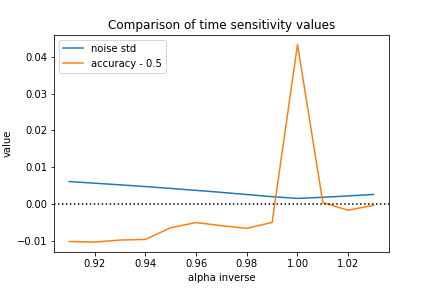
\includegraphics[width=.4\textwidth]{alpha comparison.png}
\centering
\end{figure}

بر اساس شکل در می‌یابیم نقاطی که در پیش‌بینی جهت
$\tilde{r}_n$
بیشترین دقت را دارند (از تشخیص تصادفی فاصله دارند و در عین حال انحراف معیار نویزشان کم است) عبارت‌اند از
$0.94$
و
$1$.
از طرفی کمترین انحراف معیار نویز، همانطور که پیش بینی شده بود، در حوالی 
$1$
رخ می‌دهد. پس اگر به دنبال مقداری غیر بدیهی (مخالف
$1$)
هستیم،
$\alpha=0.94$
گزینه مناسبی است. (توجه می‌کنیم که نیمه عمر چنین انتخابی حدود ۱۲ است، یعنی حساسیت مدل به داده هر لحظه حدود دو برابر حساسیت آن به داده ۱۲ کندل قبل است!)

هم‌چنین در ادامه تصویری از هیستوگرام نویز تعدادی از انتخاب‌های
$\alpha$
قابل مشاهده است.

\begin{figure}
\subfloat[$\alpha^{-1} = 0.93$]{\includegraphics[width = 2in]{Errors Histogram [Weighted (93\%) Linear Model with Control].png}} 
\subfloat[$\alpha^{-1} = 0.94$]{\includegraphics[width = 2in]{Errors Histogram [Weighted (94\%) Linear Model with Control].png}} 
\subfloat[$\alpha^{-1} = 0.95$]{\includegraphics[width = 2in]{Errors Histogram [Weighted (95\%) Linear Model with Control].png}} \\
\subfloat[$\alpha^{-1} = 0.96$]{\includegraphics[width = 2in]{Errors Histogram [Weighted (96\%) Linear Model with Control].png}} 
\subfloat[$\alpha^{-1} = 0.97$]{\includegraphics[width = 2in]{Errors Histogram [Weighted (97\%) Linear Model with Control].png}} 
\subfloat[$\alpha^{-1} = 0.98$]{\includegraphics[width = 2in]{Errors Histogram [Weighted (98\%) Linear Model with Control].png}} 
\label{alpha_values}
\centering
\end{figure}
\end{مشاهده}

\begin{نتیجه}
در شکل زیر می‌توان خروجی فیلتر کالمن را بر روی مدل خطی حساس به زمان ( با
$\alpha^{-1} = 0.94$)
در هر لحظه به ازای یک پنجره خاص زمانی مشاهده کرد.

\begin{figure}[h]
\includegraphics[width=1\textwidth]{Returns and Kalman Filtering [Weighted (94\%) Linear Model with Control]}
\centering
\end{figure}
\end{نتیجه}





\subsubsection{مدل ۴: دینامیک خطی با ماتریس چگال}
در مدل‌های قبل، برای سهولت در محاسبه و سادگی مدل، فرض کردیم ماتریس‌های
$F_n$
و
$G_n$
تنک هستند. در این مدل، بدون تغییر فرض خطی بودن دینامیک مساله، فرض تنک بودن
$F_n$
و
$G_n$
را حذف می‌کنیم. در این صورت هرچند واریانس نویز تقریب آخرین بازدهی افزایش می‌یابد، اما با توجه به اینکه حالت تنک معادله خطی زیر، یک حالت خاص از معادله کلی است، انتظار داریم مساله بهینه‌سازی بتواند جواب‌های پایدارتری تولید کند. فایده دستگاه‌های خطی با نویز
$w_n$
بالاتر ولی پایداری بیشتر ان است که در بازارهای مالی به طور طبیعی مقدار بسیار زیادی نویز غیر قابل کنترل وجود دارد، و با پایدارتر کردن مدل، به ذات دینامیک مساله بهتر دسترسی داریم. (با فرض شبیه به خطی بودن این دینامیک)






% --------------------------------------------- %
\section{فیلتر کالمن تعمیم‌یافته}
% --------------------------------------------- %

\subsection{تعریف}
\subsection{پیاده‌سازی}
\subsubsection{مدل ۵: دینامیک درجه ۲ بدون کنترل}
\subsubsection{مدل ۶: دینامیک درجه ۲ همراه با کنترل خطی}
\subsubsection{مدل ۷: دینامیک شبکه عصبی}
\subsubsection{مدل ۸: دینامیک مشتق‌ناپذیر}


\section{فیلتر کالمن سریع}


\section{فیلتر کالمن با چند مدل}
\subsection{جمع‌بندی مدل‌های ارایه شده}
\subsection{تعمیم فیلتر کالمن به چند مدل موازی}
\subsubsection{تعمیم ضرایب کالمن}
\subsubsection{ترکیب چند فیلتر}

\section{ارجاع و منابع}
\Latincite{Sung}


\bibliographystyle{alpha-persian}
\bibliography{main}


\end{document}